% Setup - do not change
\documentclass[11pt]{article}
\usepackage[top=0.9in, left=0.9in, bottom=0.9in, right=0.9in]{geometry} 
\usepackage{parskip}

\usepackage[english]{babel}
\usepackage[utf8]{inputenc}
\usepackage{amsmath,amsthm,amssymb,graphicx,pdfpages,lipsum,hyperref}
\usepackage[none]{hyphenat}
\usepackage{csquotes}

\setlength\parindent{0pt}
%%%%%%%%%%%%%%%%%%%%%%%%%%%%%%%%%%%%%%%%%%%%%%%%%%%%%%%%%%%%%%%%%%%
% add other packages here if required

%% Bibliography are specified in this file. You can also choose inline bib style if you want to. But make sure your citation style is consistent (and proper)
% For more details on citation: https://library.unimelb.edu.au/recite
\usepackage[sorting = none]{biblatex}
\usepackage{soul}
\addbibresource{references.bib}

%%%%%%%%%%%%%%%%%%%%%%%%%%%%%%%%%%%%%%%%%%%%%%%%%%%%%%%%%%%%%%%%%%%

\title{\textbf{The Effect of Weather, Population, and Property Price on the Demand for Yellow Taxis in New York City}}
\author{
Haiyang(Henry) Huang \\
Student ID: 1071147 \\
\href{https://github.com/MAST30034-Applied-Data-Science/mast30034-project-1-HenryHuang2}{Github repo with commit}
}

\begin{document}
\maketitle

\section{Introduction}
New York City, the most populous mega-city in the world \cite{nycintro}, is famous for its fast-paced lifestyle and busy traffic. Under such a background, the demand for efficient transportation is enormous. The New York City Taxi and Limousine Commission (TLC) has constantly updated trip records for multiple types of taxi and for-hire vehicles since 2009. This report will be based on the yellow taxi data in 2019\cite{tlcdata}, which contains a total number of 84,598,444 rows and 19 attributes.


The research goal of the report is to investigate the \textbf{effect of weather}, \textbf{regional population}, and \textbf{regional price of the property} on the demand for yellow taxis in New York. \ul{This report will assume that all the datasets are correct and validated}.

\section{Dataset}
\subsection{Taxi Type}
As one of the most iconic and traditional taxis in New York, \textbf{the medallion(yellow) taxi is the subject of this study} because it is flexible for the driver to pick up a passenger in any borough.
\subsection{Date Range}
New York has been affected by the COVID-19 pandemic since March 1st, 2020 \cite{covidintro}. As a result, the volume of trips declined drastically. To avoid the unexpected influence of the pandemic, \textbf{data from Jan 2019 to Dec 2019 are chosen to be the training set}, and \textbf{data from Jan 2020 to Feb 2020 are chosen to be the testing set} \cite{tlcdata}. 
\subsection{External Data}
There are 3 external datasets employed in this research. The first one is the Population By Neighborhood Tabulation Areas (NTA) from the NYC OpenData \cite{populationdata}, which contains useful information on populations in each NTA. This dataset also comes with a shapefile of NTA, which can help us to estimate the population in each taxi zone. The second one is the Annualized Sales Update data from the Department of Finance, NYC \cite{propertydata}. It provides information on property sale records in NYC which allows us to determine the average price of property per square foot for each zone. The last dataset is the daily weather in New York provided by Visual Crossing Corporation \cite{weatherdata}.
\subsection{Hypothesis}
Our hypothesis is that population will have a positive effect on the number of trips because more customers mean a larger market. Also, the property price is reflective of one's social-economic background, which can tell an interesting story about the tendencies of taking taxis of people from different financial backgrounds. Finally, we believe that weather will have a certain effect on the number of trips. For example, unexpected precipitation may increase the demand for taxis.
\section{Target Audience}
The target audiences of this report are Medallion taxi drivers, taxi companies, and New York City Taxi and Limousine Commission. 
\section{Preprocessing}
\subsubsection{Taxi data}
\begin{enumerate} 
    \item Drop the attributes that we are not interested in.
    \item Drop the rows with null passenger count and RatecodeID.
    \item Remove data that are not in 2019/2020 depending on which dataset we are dealing with.
    \item Remove outliers that are 3 standard deviations away from the mean (z-score method).
    \item RateCodeID should be one of the integers in the range of 1-6.
    \item Remove trips that are not paid by credit card or cash.
    \item Remove rows with zero Passenger count.
    \item Remove trips that start or end at zone 264 and 265 as they are unknown zone.
    \item Extract the pick-up and drop-off month in case of cross-month trips.
    \item Aggregate the number of trips by (PULocationID, PUMonth) and (DOLocationID, DOMonth)
\end{enumerate}
\subsection{Property price data}
\begin{enumerate} 
    \item Remove outliers that are 1.5 IQR away from Q1 or Q3
    \item Select rows that are dated before February 29, 2020 and after January 1, 2019
    \item Remove rows with sale price less than \$9999
    \item Remove rows with gross square feet less than 9 sq. ft
    \item Retain rows with building class starting with A or B or C or D or H where these are the building class type for accommodations (e.g. A refer to ONE FAMILY DWELLINGS)
    \item Retain rows where the building class is unchanged throughout the life of the building because building class might have an effect on price.
    \item Aggregate the mean price of properties in each neighborhood.
    \item Link the property price data with taxi zones data based on the similarity between neighborhood name and service zone name.
\end{enumerate}
\subsection{Population data}
\begin{itemize}
    \item Assume the population in each neighborhood is evenly distributed, use the shapefiles to compute the overlapping area of taxi zones and neighborhoods, then sum all the segments of the population for each taxi zone. \[ Population_i = \sum_j Population_j * P(TaxiZone_i\cap Neighborhood_j)\]
\end{itemize}
\subsection{Weather data}
\begin{itemize}
    \item Select Attributes that are thought to be relevant such as "feels like" temperature, precipitation, and snow. The rationale behind choosing "feels like" temperature rather than the actual temperature is because "feels like" conveys a more direct message of how people feel about the temperature, which may impact their decision of whether or not to hail a cab.
    \item Group the data by month and take the mean of selected attributes.
\end{itemize}
\section{Preliminary Data Analysis}
\subsection{Monthly trip count}
Apparently, from Figure \ref{fig:monthlytripcount}, there is a trend of downturn between June and August, indicating that the number of trips can be negatively correlated with temperatures. But \textbf{there is no causal relationship between temperature and number of trips in a month}. In addition to weather data, we need more data to explain the phenomenon, for example, important events in New York City during that time.
\begin{figure}[h]
    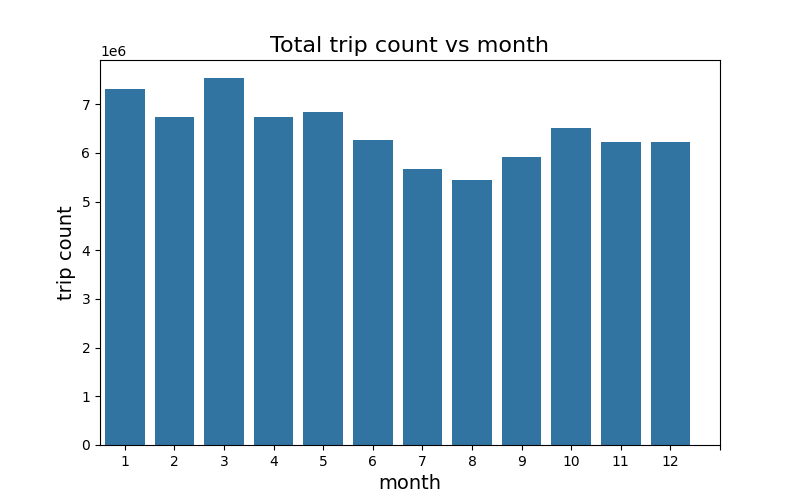
\includegraphics[width=0.7\textwidth]{plots/trip_count_vs_month.png}
    \centering
    \caption{Number of Trips vs. Month}
    \label{fig:monthlytripcount}
\end{figure}
\subsection{Distribution of total trip count}
As we can see from Figure \ref{fig:distributionoftripcount}, the total number of trip counts per location is extremely right-skewed, which implies a log transformation is suitable.
\begin{figure}[h]
    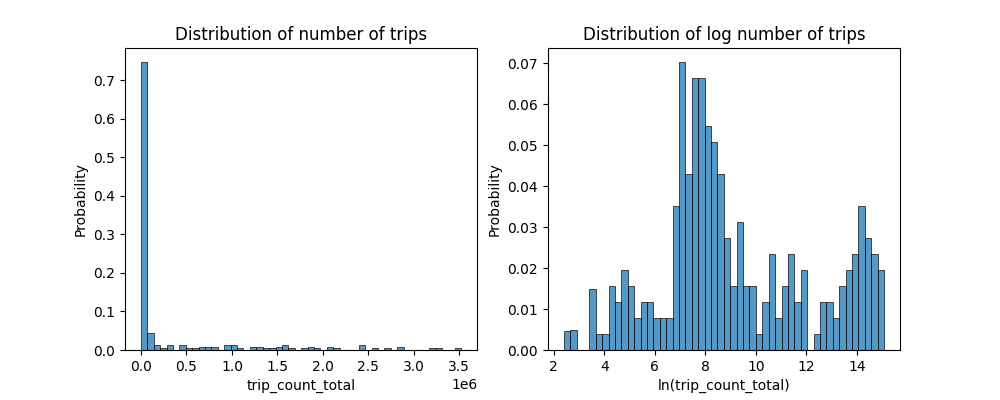
\includegraphics[width=\textwidth]{plots/trip_count_distribution.png}
    \centering
    \caption{Distribution of Number of Trips vs. Log-transformed}
    \label{fig:distributionoftripcount}
\end{figure}
\subsection{Correlation between features}
As shown in Figure \ref{fig:democorr}, we can see that the correlation between price per square foot and price per unit is relatively high compared to other attributes. Intuitively it makes sense because the gross square feet of a unit may not vary significantly. In contrast, the correlation between population and density is not as high as the former because there are taxi zones in Manhattan that have a small geographical area but are densely populated. 

Some highly correlated attributes are depicted in Figure \ref{fig:weathercorr}, such as average feelslike, feelslike min, and feelslike max. We will retain densely the average feelslike since it is more representative of the temperature in a month. In addition, precipitation, cloud cover, precipitation cover, and visibility are highly correlated to each other. As stated in \cite{weathermetadata}, the precipitation cover is the amount of time and the cloud cover is the percentage of the sky covered by cloud, precipitation is retained because intuitively the heaviness of rain has a greater impact on people's decisions of whether to take a cab or not. Moreover, visibility may contain some extra information about fog, smog, or some such which is not covered by other attributes. 
\subsubsection{Distribution of Attributes}
The demographic attributes are slightly right-skewed, which may imply that a log transformation can be applied \ref{fig:distributionofdemo}.
\subsubsection{Final Attributes} 
The final set of attributes for weather model are ``feelslike'', ``precip'', ``windspeed'', ``visibility'', ``snow'' and ``snowdepth''. For demographic model, the final set of attributes are ``Price\_per\_square\_feet'', ``Population\_By\_LocationID'', ``Density\_per\_hectare'', ``ln\_Price\_per\_square\_feet'', ``ln\_Population'' and ``ln\_Density\_per\_hectare''.
\begin{figure}[h]
    \centering
    \begin{minipage}{0.45\textwidth}
        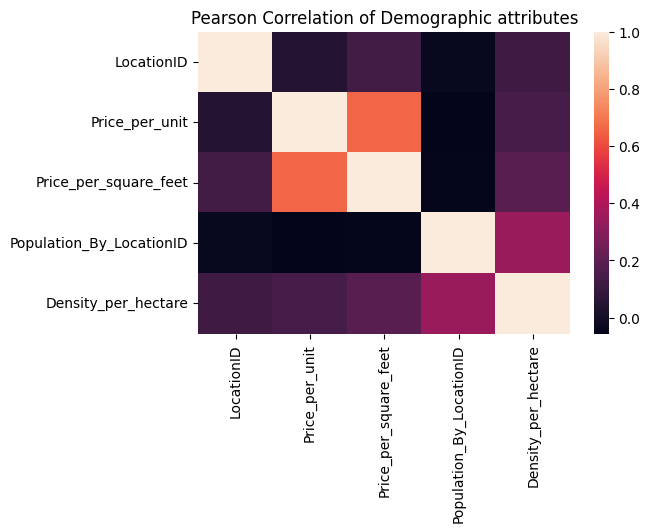
\includegraphics[width=1.2\textwidth]{plots/demo_cor.png}
        \caption{Correlations between Demographic Attributes}
        \label{fig:democorr}
    \end{minipage}\hfill
    \begin{minipage}{0.45\textwidth}
        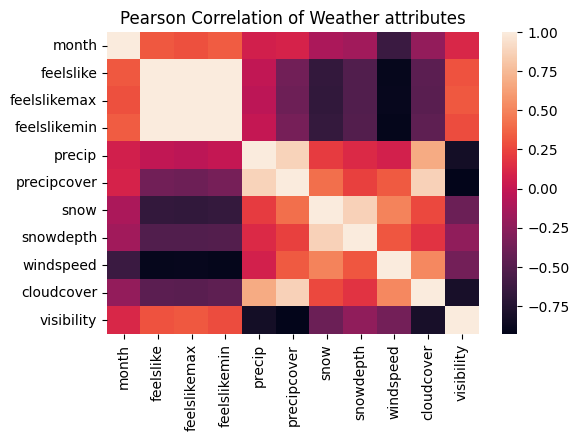
\includegraphics[width=1.2\textwidth]{plots/weather_cor.png}
        \caption{Correlations between Weather Attributes}
        \label{fig:weathercorr}
    \end{minipage}
\end{figure}
\begin{figure}[h]
    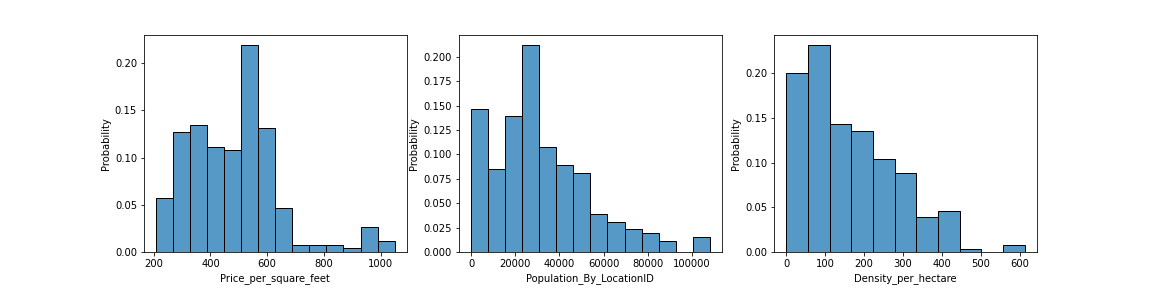
\includegraphics[width=1.15\textwidth]{plots/distribution_of_demo.png}
    \caption{Distribution of Demographic Attributes}
    \label{fig:distributionofdemo}
\end{figure}
\section{Geospatial Visualisation}
As we can see in the map \ref{fig:pickup}, the number of pickups in a location is very similar to the number of dropoffs, which is not surprising. The most popular pick-up and drop-off locations are around Manhattan, which suggests a positive relationship between the number of trips and the density of pick-up or drop-off locations. In addition, the number of pickups in JFK and Laguardia airports is relatively higher than their neighboring zones. For the purpose of this report, the three airports are removed because the number of pickups and dropoffs is affected by their usage. 
\begin{figure}[h]
    \centering
    \begin{minipage}{0.45\textwidth}
        \centering
        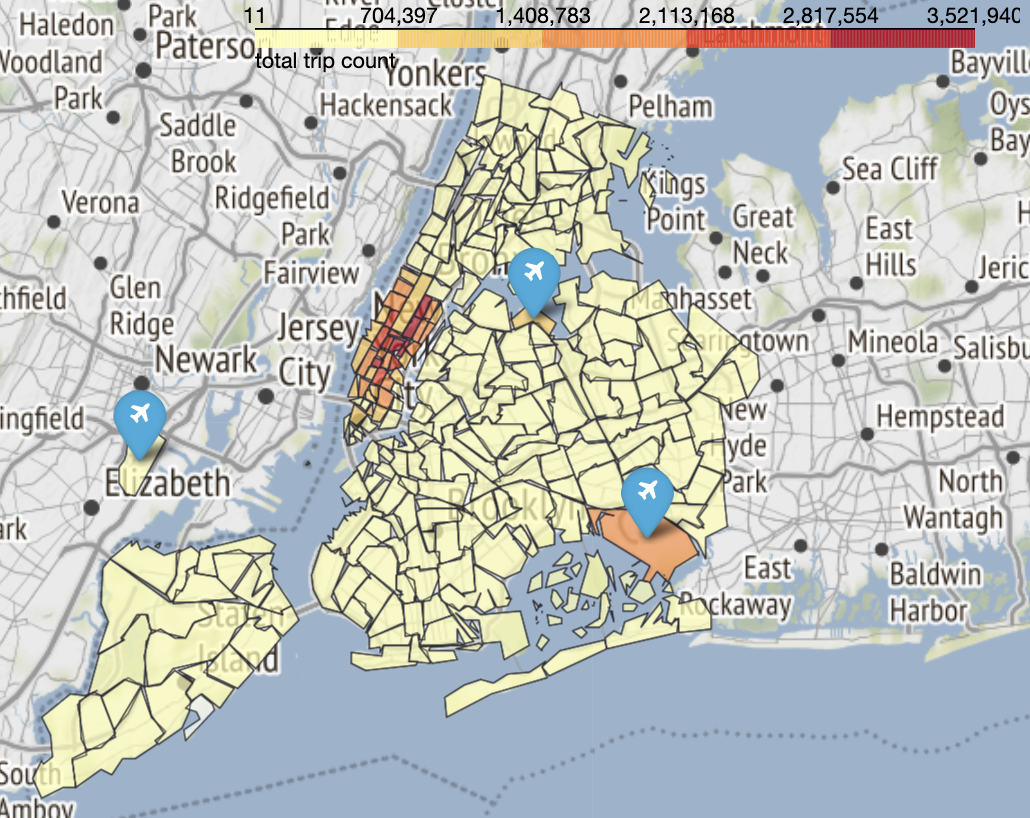
\includegraphics[width=1.2\textwidth]{plots/Screen Shot 2022-08-23 at 3.09.58 pm.png}
        \caption{Number of Pickup for all Locations in 2019}
        \label{fig:pickup}
    \end{minipage}\hfill
    \begin{minipage}{0.45\textwidth}
        \centering
        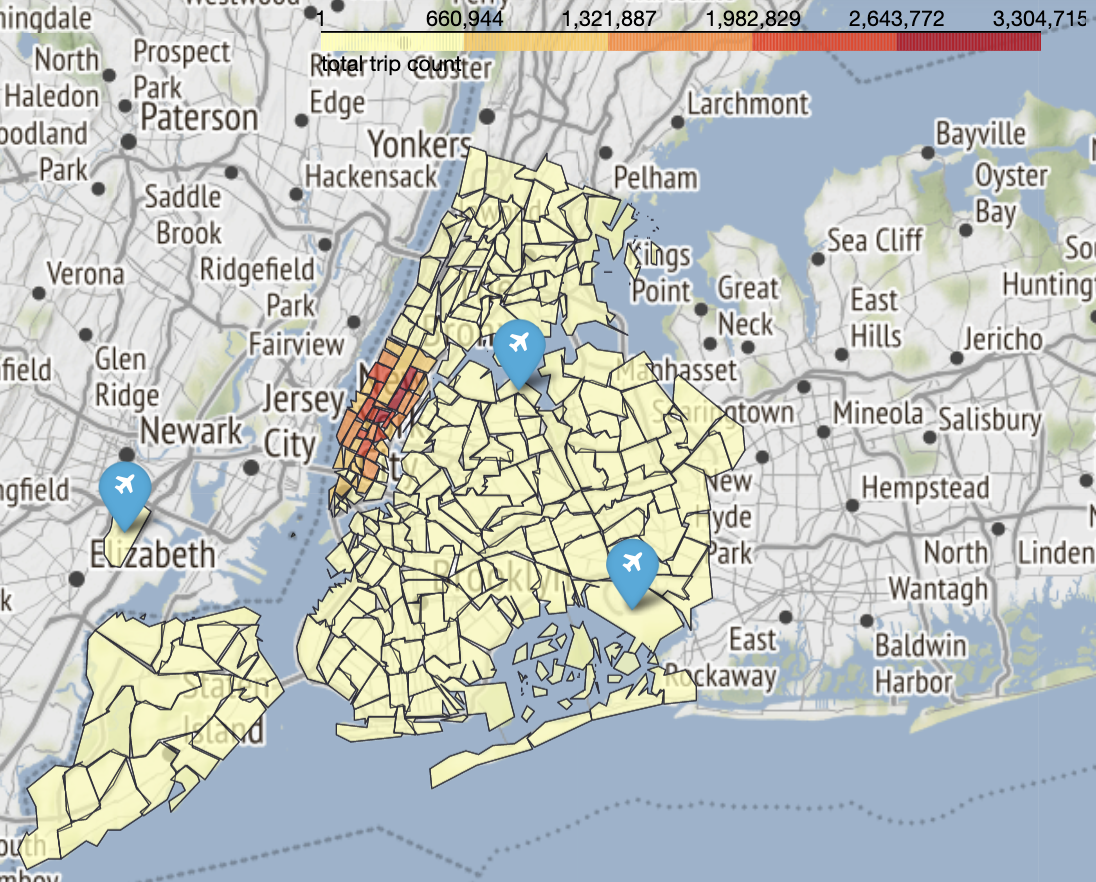
\includegraphics[width=1.2\textwidth]{plots/Screen Shot 2022-08-23 at 3.10.19 pm.png}
        \caption{Number of Dropoffs for all Locations in 2019}
        \label{fig:dropoff}
    \end{minipage}
\end{figure}

\section{Modelling}
In this report, we will be using two contrasting models, one is the Ordinary Least Square model, and another one is Lasso Penalised regression. The reasons for choosing these two models are because they are highly interpretable and have low time complexity. These two models should be adequate to show some of the relationships between the response variables and covariates. Since they are both linear models, the linearity between the response variable and the covariates is assumed. This is checked through visualization in Figure \ref{fig:demolinearity}. In addition, we assume that there is no imperfect collinearity and independence of errors as it will affect the accuracy of our model parameters, which will lead to a false interpretation. To eliminate uninformative attributes, we make use of the step-wise selection method with AIC as the metric. The evaluation metric used are ANOVA table, $R^2$, and Root Mean Square Error. The advantage of using RMSE is that it has the same scale as the data, which can help us understand how well our regressions perform on a similar scale. Moreover, HC2 standard errors are used in ANOVA, which can avoid the effect of heteroskedasticity.

\begin{figure}[h]
    \centering
    \begin{minipage}{0.45\textwidth}
        \centering
        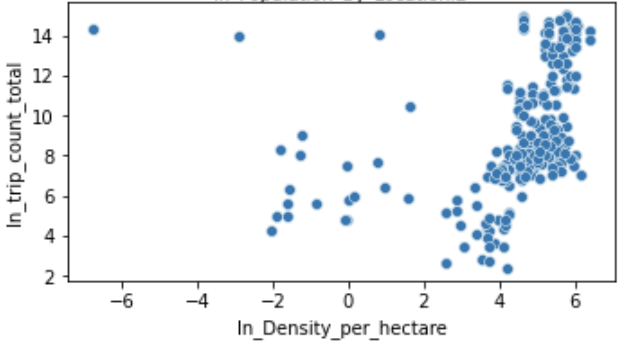
\includegraphics[width=1.2\textwidth]{plots/Screen Shot 2022-08-23 at 8.35.00 pm.png}
        \caption{Sample Linearity check of Demographic Attributes}
        \label{fig:demolinearity}
    \end{minipage}\hfill
    \begin{minipage}{0.45\textwidth}
        \centering
        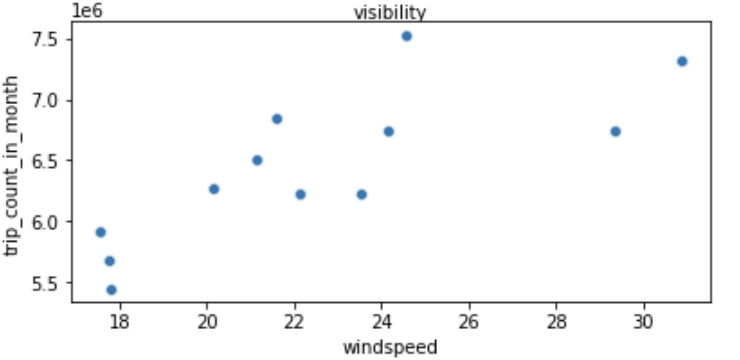
\includegraphics[width=1.2\textwidth]{plots/Screen Shot 2022-08-23 at 5.14.12 pm.png}
        \caption{Sample Linearity check of Weather Attributes}
        \label{fig:weatherlinearity}
    \end{minipage}
\end{figure}
\subsection{Effect of Weather}
\subsubsection{OLS Model}
Our initial covariates are ``feelslike'', ``precip'', ``windspeed'', ``visibility'', ``snow'' and ``snowdepth''. After a step-wise selection is performed, ``feelslike'' and ``precip'' are removed. The ANOVA table shows that all of the remaining covariates are statistically significant from 0 at 0.001 significance level\ref{fig:weatheranova}. As shown in figure \ref{fig:weathercoef}, visibility and snow have a negative effect on the number of trips. One possible explanation could be that bad weather condition makes driver harder to find a customer because people tend to stay indoors until the weather is clear. An interesting fact is that snow depth has a positive effect on the number of trips, this may happen when snow is deep and other transportation like riding bikes or walking are not suitable. The $R^2$ of the model is 0.939 which is much higher than the baseline model with a 0 R squares (the result of the baseline model is now shown here due to the limitations of report length), however, the RMSE of 1.597e+06 is very high as well, meaning that our model is not very predictive.
\begin{figure}[h]
    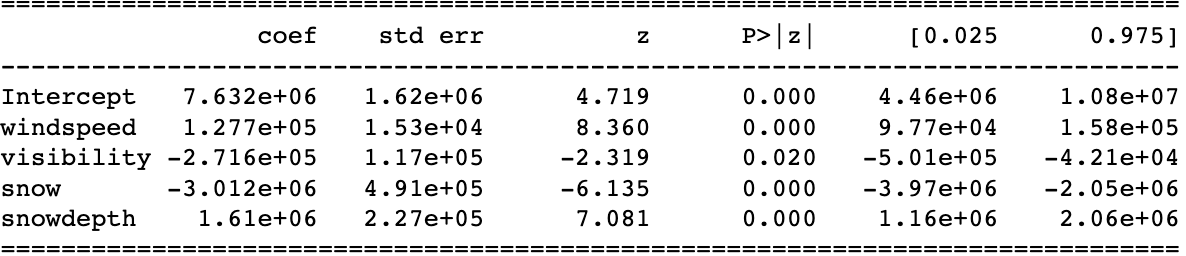
\includegraphics[width=0.8\textwidth]{plots/olsweathercoef.png}
    \centering
    \caption{OLS Model Coefficient of Weather}
    \label{fig:weathercoef}
\end{figure}
\begin{figure}[h]
    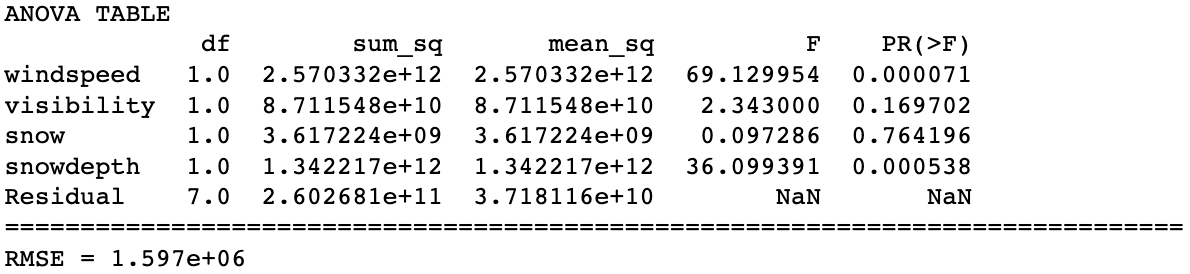
\includegraphics[width=0.8\textwidth]{plots/anovaweather.png}
    \centering
    \caption{ANOVA Table of Weather}
    \label{fig:weatheranova}
\end{figure}
\subsubsection{Lasso Model}
The final Lasso regression model is as followed: $trip\_count\_in\_month = 1.03\times10^6 - 7.78\times10^2feelslike -7.70\times10^4precip + 1.20\times10^5windspeed - 4.25\times10^5visibility -3.08\times10^6snow + 1.63\times10^6snowdepth.$ Noting that the coefficients of the Lasso model are quite different from the OLS model, this is because the Lasso regression does not shrink any of the covariates to zero, which implies that there is no imperfect multicollinearity between covariates. The $R^2$ of Lasso is 0.9478, which is higher than the OLS model. However, the RMSE has increased from 1.597e+06 to 1.622e+06, which indicates a trend of overfitting.

\subsection{Pickup and Dropoff Model}
From table \ref{tab:pickupanova} and table \ref{tab:dropoffanova}, we can see that all three covariates are statistically significant from 0 at 0.01 significance level. Amongst the three covariates, the log of density per hectare has the highest mean sum of squares, which means that there is a large variation in the number of pickups/dropoffs due to the population density of a zone. Keeping other covariates unchanged, the pickup model indicates that a 1\% increase in density per hectare is expected to result in a 2.1149\% increase in the pickup number in a zone. For the dropoff model, this number rises to 2.5174\%. It is worth noting that, a 1\% increase in total population in a zone is associated with a 1.5140\% and 1.8432\% decrease in the number of pickups and dropoffs, respectively. This suggests that our models are biased toward Manhattan, which is the most densely populated borough in New York City. In addition, both models show a trend of increase in the number of trips as the property price increase, but the p-values are relatively high compared to the other two variables. Therefore, we cannot make a confident conclusion about the effect of the property price. The $R^2$ is 0.559 for the pickup model and 0.513 for the dropoff model, which means that our model is able to explain around 50\% of variations in the response variable. The RMSE for the pickup model is 3.179, which suggests that our model is not particularly useful for prediction. The RMSE for the dropoff model is 2.445. In comparison to the pickup model, the dropoff model is able to predict more accurate results.

\section{Recommendations}
The first recommendation is for the taxi company. Based on our findings, regions with high population density have higher demand. This information can be used to allocate taxis for higher profitability, or plan the location of a new branch office to make shifts smoother. The second recommendation is for medallion taxi drivers and TLC. As the model suggests, bad weather condition like heavy snow or low visibility is associated with a decrease in the number of trips, which will have a detrimental effect on taxi drivers' income. TLC is encouraged to find a solution to cope with weather contingencies, for example, by providing this information to taxi drivers and advising them to re-arrange their working time in a more efficient way.

\begin{table}
\centering
\begin{tabular}{||c c c c c||}
 \hline
 Attribute & Coef & std err & z & P\textgreater\|z\| \\ [0.5ex]
 \hline\hline
 Intercept & -1.8982 & 2.676 & -0.709 & 0.478 \\ 
 \hline
 ln\_Price\_per\_square\_feet & 2.6515 & 0.401 & 6.617 & 0.000\\
 \hline
 ln\_Population\_By\_LocationID & -1.5140 & 0.144 & -10.507 & 0.000\\
 \hline
ln\_Density\_per\_hectare & 2.1149 & 0.164 & 12.880 & 0.000\\
 \hline
\end{tabular}
  \caption{Coefficient of Pickup Model}
  \label{tab:pickup}
\begin{tabular}{||c c c c c c||}
 \hline
 Attribute & df & sum\_sq & mean\_sq & F & PR\textgreater(F) \\ [0.5ex]
 \hline\hline
 ln\_Price\_per\_square\_feet & 1 & 429.055 & 429.055 & 103.215 & 1.55e-20\\
 \hline
 ln\_Population\_By\_LocationID & 1 & 37.956 & 37.956 & 9.131 & 2.77e-03\\
 \hline
ln\_Density\_per\_hectare & 1 & 857.187 & 857.187 & 206.207 & 1.54e-34\\
 \hline
 Residual & 251 & 1043.389 & 4.157 & & \\ 
 \hline
\end{tabular}
  \caption{ANOVA Table of Pickup Model}
  \label{tab:pickupanova}
\end{table}
\begin{table}
\centering
\begin{tabular}{||c c c c c||}
 \hline
 Attribute & Coef & std err & z & P\textgreater\|z\| \\ [0.5ex]
 \hline\hline
 Intercept & 5.7480 & 4.198 & 1.369 & 0.171 \\ 
 \hline
 ln\_Price\_per\_square\_feet & 1.2721 & 0.623 & 2.042 & 0.041\\
 \hline
 ln\_Population\_By\_LocationID & -1.8432 & 0.171 & -10.809 & 0.000\\
 \hline
ln\_Density\_per\_hectare & 2.5174 & 0.186 & 13.537 & 0.000\\
 \hline
\end{tabular}
  \caption{Coefficient of Dropoff Model}
  \label{tab:dropoff}
\begin{tabular}{||c c c c c c||}
 \hline
 Attribute & df & sum\_sq & mean\_sq & F & PR\textgreater(F) \\ [0.5ex]
 \hline\hline
 ln\_Price\_per\_square\_feet & 1 & 72.672 & 72.672 & 13.796 & 2.513e-04\\
 \hline
 ln\_Population\_By\_LocationID & 1 & 36.537 & 36.537 & 6.936 & 8.973e-03\\
 \hline
ln\_Density\_per\_hectare & 1 & 1278.341 & 1278.341 & 242.685 & 8.973e-03\\
 \hline
 Residual & 250 & 1316.872 & 5.267 & & \\ 
 \hline
\end{tabular}
  \caption{ANOVA Table of Dropoff Model}
  \label{tab:dropoffanova}
\end{table}

\clearpage

\printbibliography

\end{document}